
In this section, the results of the regression cases (burnup, enrichment, and
time since irradiation) are presented. For each prediction parameter, the plot
format described in Figure \ref{fig:detdemo} is used to show both the
\gls{MAPE} and \gls{MAE} for each of the three energy window lists.  However,
while seeing the performance decrease with all three algorithms on the same
plot is helpful for getting a bigger picture of the results, a more detailed
visual is also helpful. Box plots provide this increased statistical detail and
a direct comparison of mean and median error for each data point. There are the
same "goal" lines (blue lines) and baselines (red lines), but they are flipped
since the axis is no longer negative.  There is one plot for each algorithm for
a given energy window list-based set of detector training sets.  Because these
are box plots, they are not oriented to the "higher is better" standard of the
\textit{y}-axis of the original prediction performance plots. Additionally, the
full knowledge cases (the 29 nuclide masses, and the 32, 12, and 7 nuclide
activities sets) are not able to be represented on the same scale as the
detector training set results, so they are excluded from the box plot figures. 

\subsubsection{Burnup Regression}

\begin{figure}[!htb]
  \centering
  \begin{subfigure}[b]{\textwidth}
    \centering
    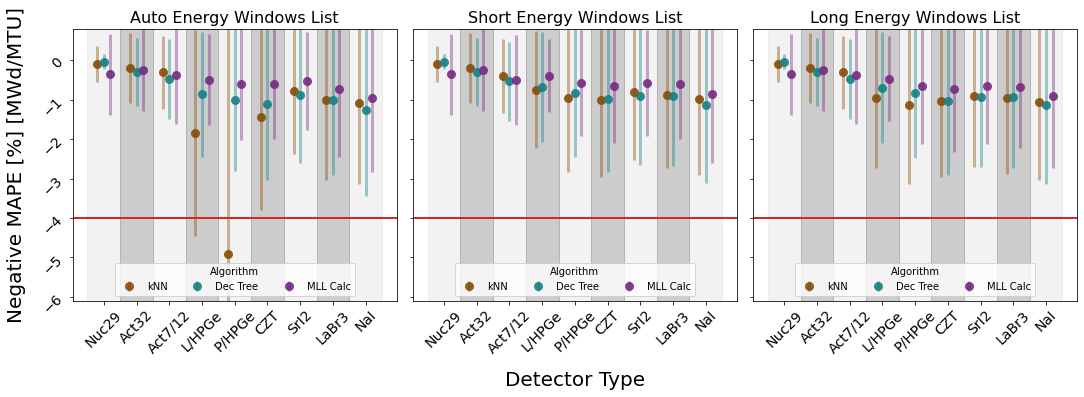
\includegraphics[width=\textwidth]{./chapters/exp2/detector_preds_wrt_enlist_MAPE_burn.png}
    \caption{Burnup prediction performance measured by \gls{MAPE}.}
    \label{fig:burnA}
  \end{subfigure}
  \vskip\baselineskip
  \begin{subfigure}[b]{\textwidth}
    \centering
    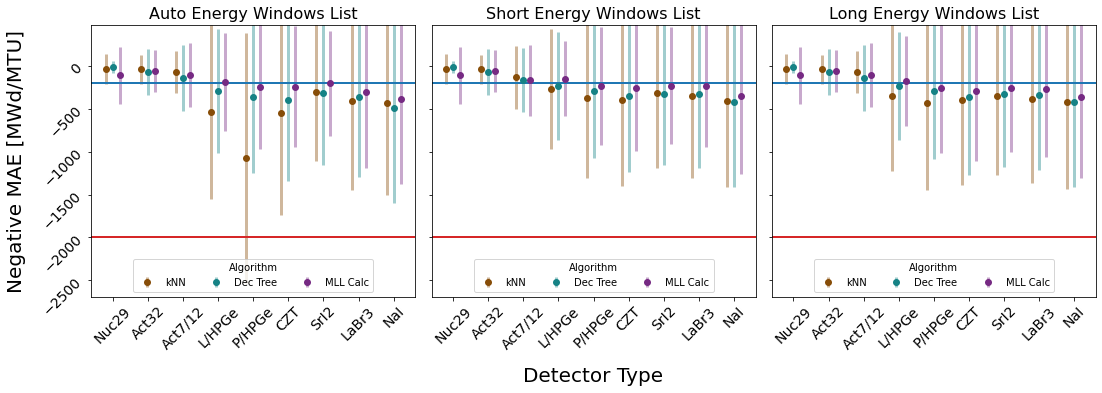
\includegraphics[width=\textwidth]{./chapters/exp2/detector_preds_wrt_enlist_MAE_burn.png}
    \caption{Burnup prediction performance measured by \gls{MAE}.} 
    \label{fig:burnB}
  \end{subfigure}
  \caption{Prediction performance of burnup with respect to decreasing detector 
           energy resolution for three types of processed gamma spectra.}
  \label{fig:burn}
\end{figure}

The goal lines and baselines for the burnup plots in Figure \ref{fig:burn} were
all chosen by the performance of algorithms at a reference point of 20\%
training set error for the 29 nuclide mass training set in in Figures
\ref{fig:randerrB} and \ref{fig:randmaeA}.  For Figure \ref{fig:burnA}, the
blue line is at -1\% , which corresponds to the \gls{MLL} performance at the
reference point.  The red baseline is at -4\%, which is the lowest performance
of all three algorithms at the reference point.  For Figure \ref{fig:burnB},
the blue line is at $-300\:MWd/MTU$, and the red baseline is at
$-1000\:MWd/MTU$.  These also correspond to \gls{MLL} and \textit{k}-nearest
neighbors, respectively, at the reference point in Figure \ref{fig:randmaeA}.
The same lines are present in Figure \ref{fig:burnbox}, but instead are
positive values so the red line is on top.  \todo[inline]{the other two cases
below have arbitrary baselines for a more discriminatory discussion, maybe that
would be useful to do here too. leaving discussion for later}

\begin{figure}[!hp]
  \centering
  \begin{subfigure}[b]{\textwidth}
    \centering
    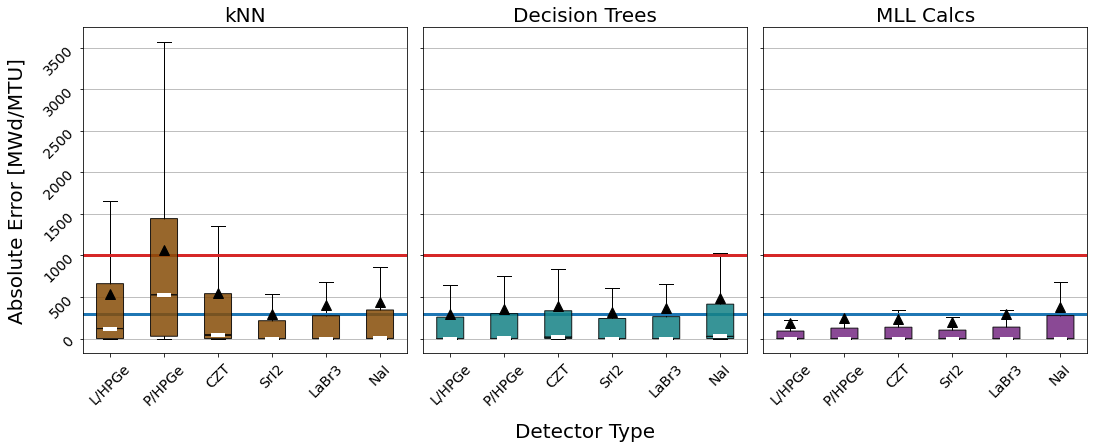
\includegraphics[width=0.92\textwidth]{./chapters/exp2/abserror_boxplots_auto_burn.png}
    \caption{Burnup prediction error box plots for auto energy windows list.}
    \label{fig:burnboxA}
  \end{subfigure}
  \vskip\baselineskip
  \begin{subfigure}[b]{\textwidth}
    \centering
    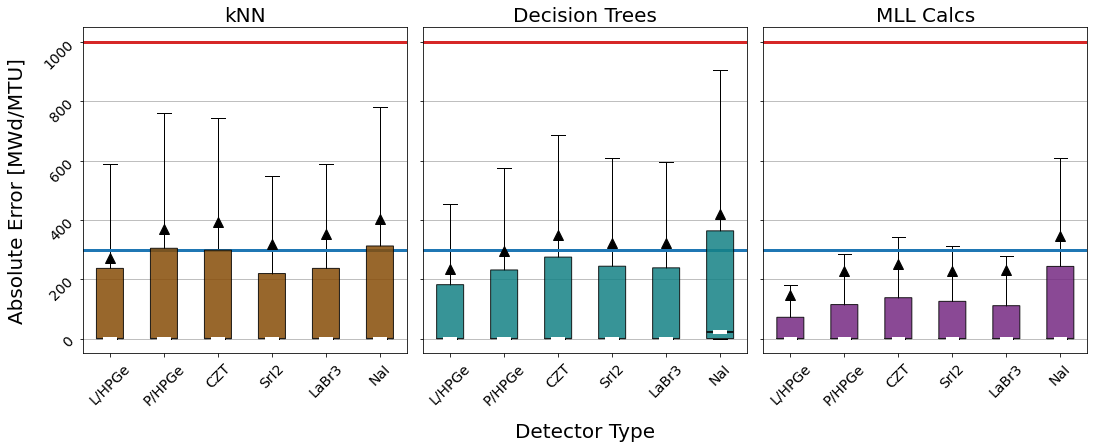
\includegraphics[width=0.92\textwidth]{./chapters/exp2/abserror_boxplots_short_burn.png}
    \caption{Burnup prediction error box plots for short energy windows list.}
    \label{fig:burnboxB}
  \end{subfigure}
  \vskip\baselineskip
  \begin{subfigure}[b]{\textwidth}
    \centering
    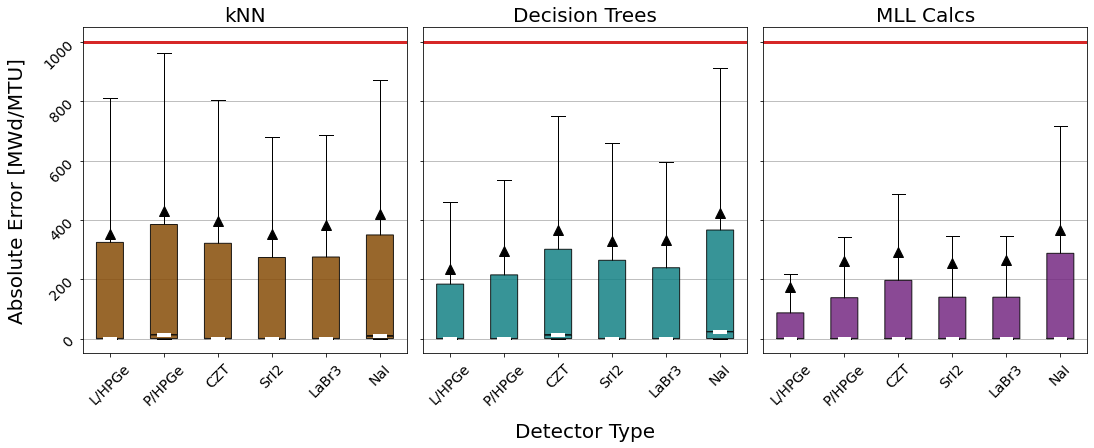
\includegraphics[width=0.92\textwidth]{./chapters/exp2/abserror_boxplots_long_burn.png}
    \caption{Burnup prediction error box plots for long energy windows list.}
    \label{fig:burnboxC}
  \end{subfigure}
  \caption{Prediction performance of burnup for six detectors as shown by box 
           plots.}
  \label{fig:burnbox}
\end{figure}

\begin{figure}[!hp]
  \centering
  \begin{subfigure}[b]{\textwidth}
    \centering
    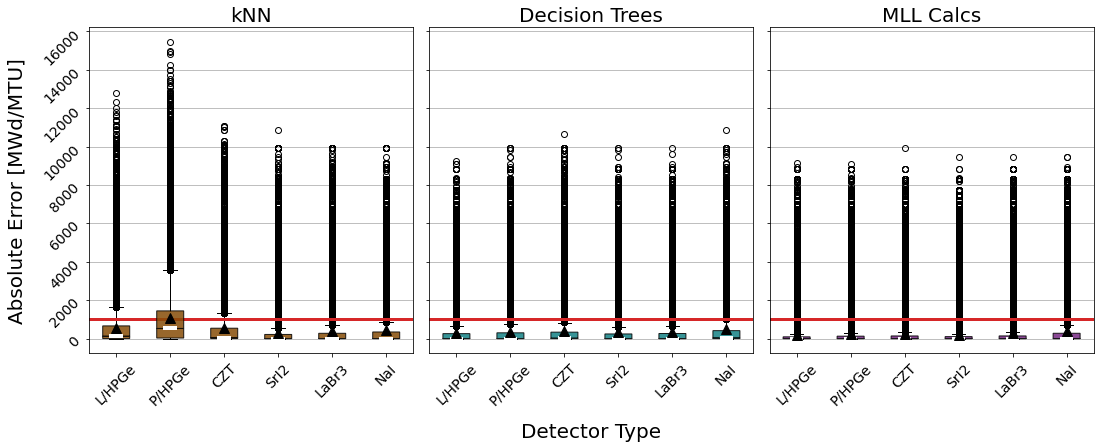
\includegraphics[width=0.92\textwidth]{./chapters/exp2/abserror_boxplots_outliers_auto_burn.png}
    \caption{Burnup prediction error box plots for auto energy windows list.}
    \label{fig:burnboxflyA}
  \end{subfigure}
  \vskip\baselineskip
  \begin{subfigure}[b]{\textwidth}
    \centering
    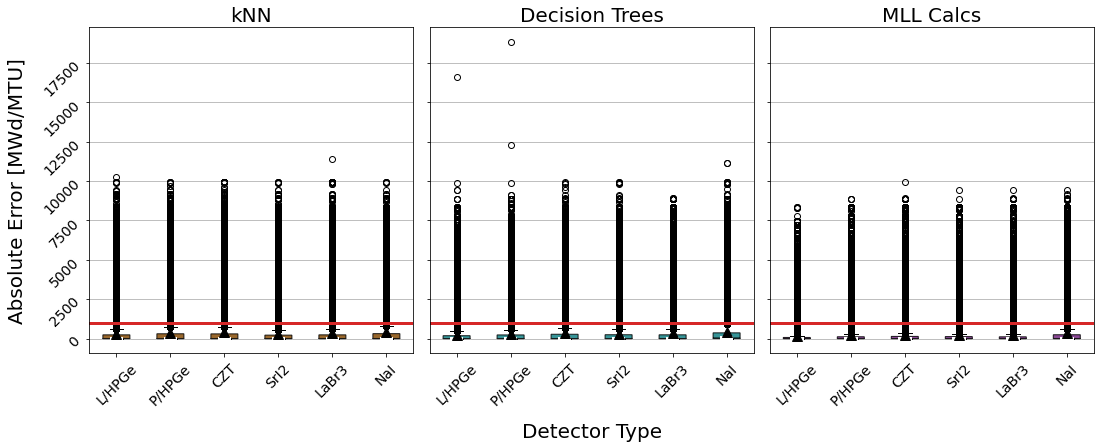
\includegraphics[width=0.92\textwidth]{./chapters/exp2/abserror_boxplots_outliers_short_burn.png}
    \caption{Burnup prediction error box plots for short energy windows list.}
    \label{fig:burnboxflyB}
  \end{subfigure}
  \vskip\baselineskip
  \begin{subfigure}[b]{\textwidth}
    \centering
    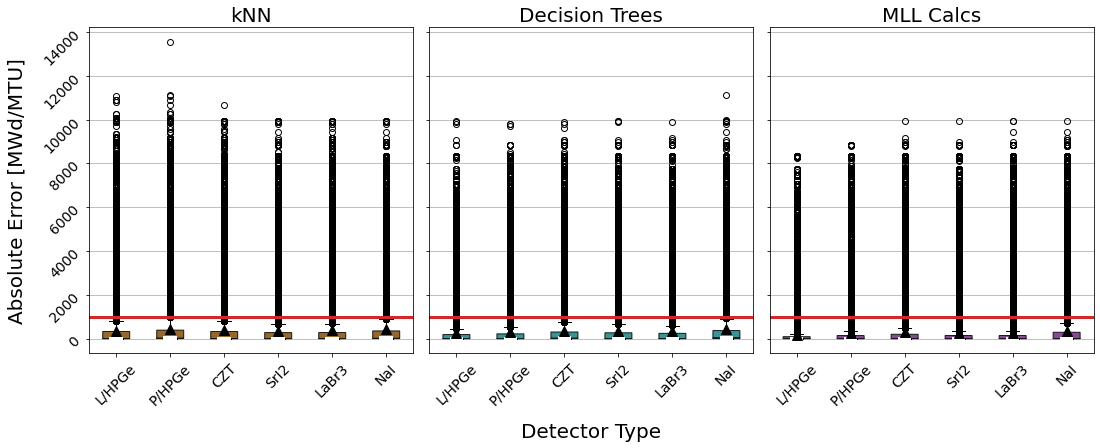
\includegraphics[width=0.92\textwidth]{./chapters/exp2/abserror_boxplots_outliers_long_burn.png}
    \caption{Burnup prediction error box plots for long energy windows list.}
    \label{fig:burnboxflyC}
  \end{subfigure}
  \caption{Prediction performance of burnup for six detectors as shown by box 
           plots.}
  \label{fig:burnboxfly}
\end{figure}

\subsubsection{U235 Enrichment Regression}

The goal lines for the enrichment plots in Figure \ref{fig:enri} were both
chosen by the performance of algorithms at a reference point of 20\% training
set error for the 29 nuclide mass training set in in Figures \ref{fig:randerrC}
and \ref{fig:randmaeB}.  Since the results in these two figures were much
better than the detector results, the baselines were chosen somewhat
arbitrarily.  This is partially in order to draw a line through the clustering
of the detector results.  For Figure \ref{fig:enriA}, the blue line is at -6\%
, which corresponds to the \textit{k}-nearest neighbors performance at the
reference point.  The red baseline is at -30\%, which is the previously
mentioned arbitrary choice.  For Figure \ref{fig:enriB}, the blue line is at
$-0.15\:\% U235$, and the red baseline is at $-0.6\:\% U235$.  The former
corresponds to \textit{k}-nearest neighbors at the reference point in Figure
\ref{fig:randmaeB}, and the latter is another arbitrary choice based on where
the detector results are clustering.  The same lines are present in Figure
\ref{fig:enribox}, but instead are positive values so the red line is on top.

\begin{figure}[!htb]
  \centering
  \begin{subfigure}[b]{\textwidth}
    \centering
    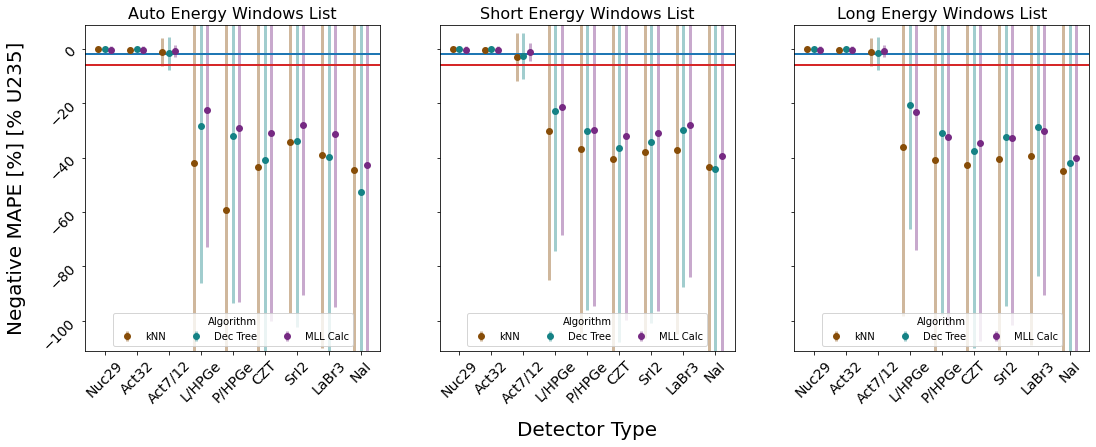
\includegraphics[width=\textwidth]{./chapters/exp2/detector_preds_wrt_enlist_MAPE_enri.png}
    \caption{\gls{U235} enrichment prediction performance measured by \gls{MAPE}.}
    \label{fig:enriA}
  \end{subfigure}
  \vskip\baselineskip
  \begin{subfigure}[b]{\textwidth}
    \centering
    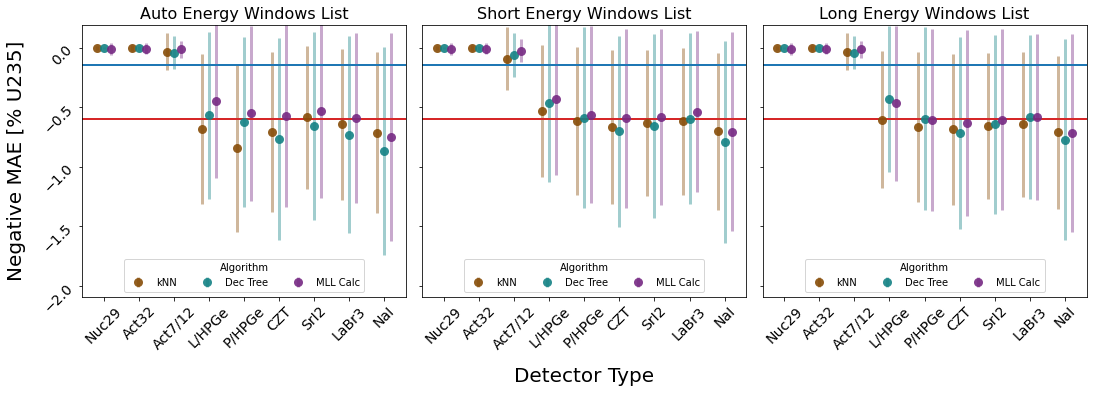
\includegraphics[width=\textwidth]{./chapters/exp2/detector_preds_wrt_enlist_MAE_enri.png}
    \caption{\gls{U235} enrichment prediction performance measured by \gls{MAE}.} 
    \label{fig:enriB}
  \end{subfigure}
  \caption{Prediction performance of \gls{U235} enrichment with respect to 
           decreasing detector energy resolution for three types of processed 
           gamma spectra.}
  \label{fig:enri}
\end{figure}

Taken as a whole, the data points in Figure \ref{fig:enri} have a distinct
shape, similar to the behavior in Figue \ref{fig:rxtr}.  The three full
knowledge cases have near-perfect enrichment prediction and the six detectors
for all three energy windows lists are nearly flat. For both Figures
\ref{fig:enriA} and \ref{fig:enriB}, the blue line is therefore not making any
meaningful discrimination. The almost even performance across detector types 
and algorithms (with exceptions) \todo{left off here}

\begin{figure}[!hp]
  \centering
  \begin{subfigure}[b]{\textwidth}
    \centering
    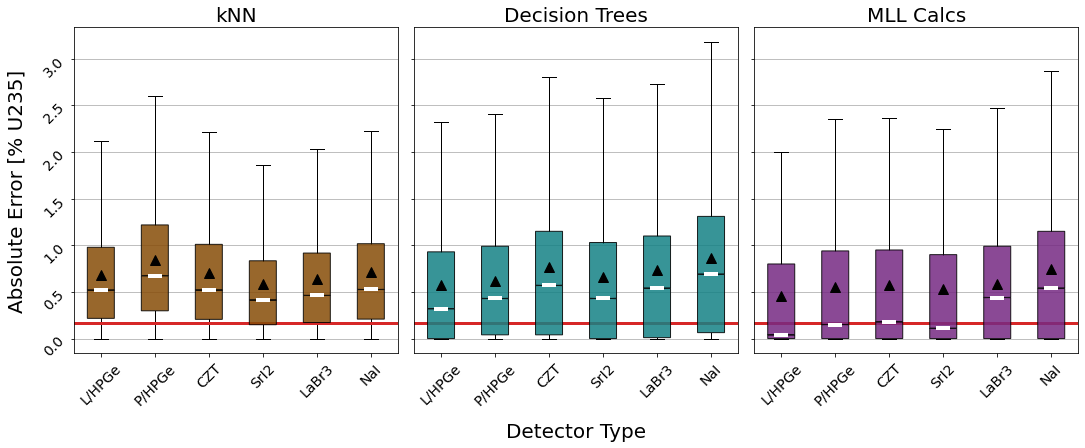
\includegraphics[width=0.92\textwidth]{./chapters/exp2/abserror_boxplots_auto_enri.png}
    \caption{\gls{U235} enrichment prediction error box plots for auto energy windows list.}
    \label{fig:enriboxA}
  \end{subfigure}
  \vskip\baselineskip
  \begin{subfigure}[b]{\textwidth}
    \centering
    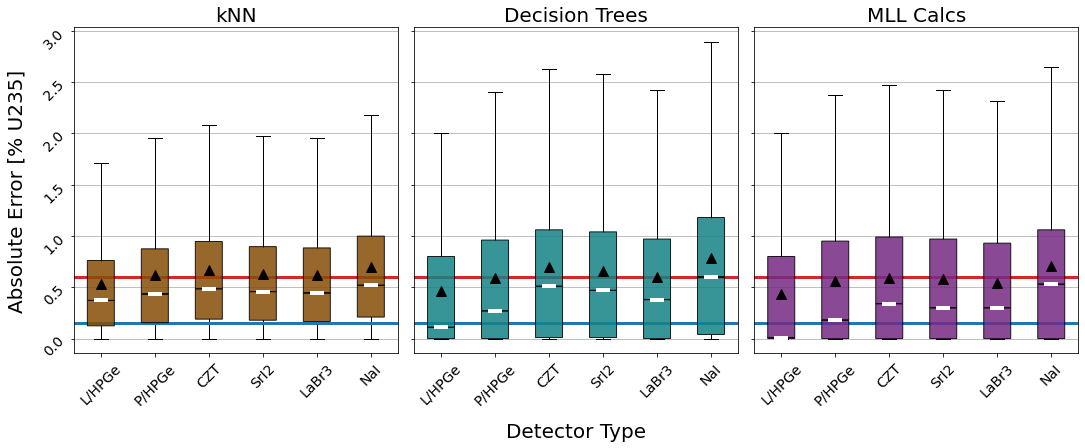
\includegraphics[width=0.92\textwidth]{./chapters/exp2/abserror_boxplots_short_enri.png}
    \caption{\gls{U235} enrichment prediction error box plots for short energy windows list.}
    \label{fig:enriboxB}
  \end{subfigure}
  \vskip\baselineskip
  \begin{subfigure}[b]{\textwidth}
    \centering
    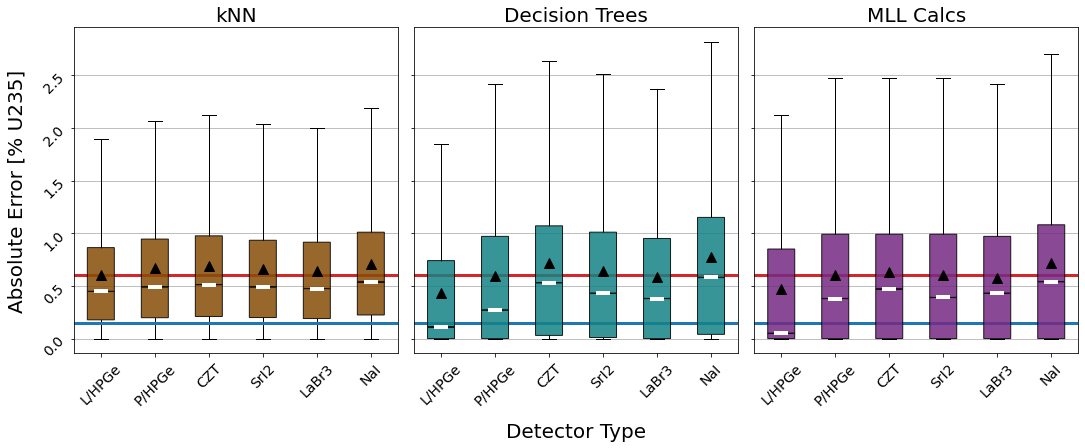
\includegraphics[width=0.92\textwidth]{./chapters/exp2/abserror_boxplots_long_enri.png}
    \caption{\gls{U235} enrichment prediction error box plots for long energy windows list.}
    \label{fig:enriboxC}
  \end{subfigure}
  \caption{Prediction performance of \gls{U235} enrichment for six detectors as 
           shown by box plots.}
  \label{fig:enribox}
\end{figure}

\begin{figure}[!hp]
  \centering
  \begin{subfigure}[b]{\textwidth}
    \centering
    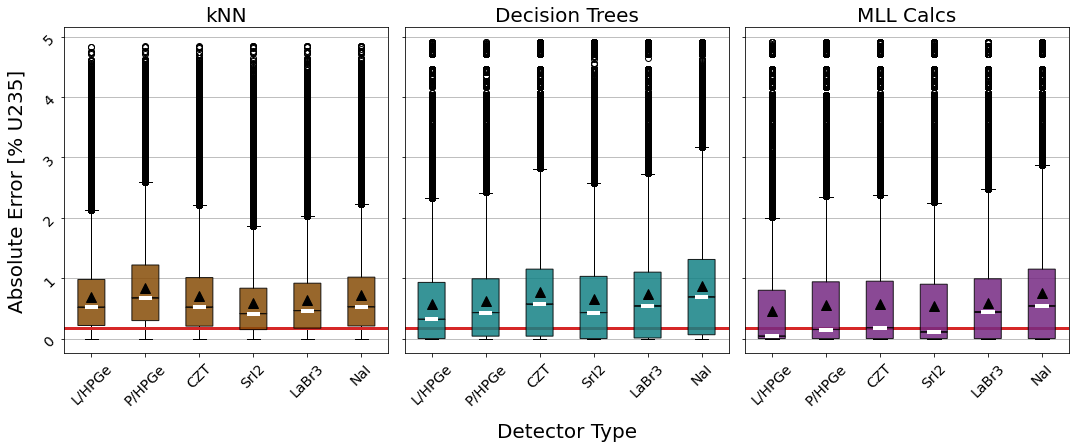
\includegraphics[width=0.92\textwidth]{./chapters/exp2/abserror_boxplots_outliers_auto_enri.png}
    \caption{\gls{U235} enrichment prediction error box plots for auto energy windows list.}
    \label{fig:enriboxflyA}
  \end{subfigure}
  \vskip\baselineskip
  \begin{subfigure}[b]{\textwidth}
    \centering
    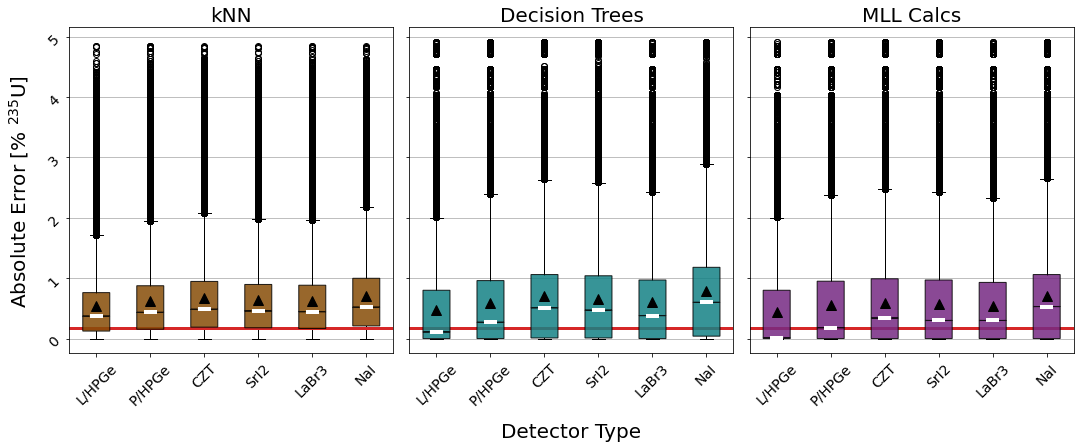
\includegraphics[width=0.92\textwidth]{./chapters/exp2/abserror_boxplots_outliers_short_enri.png}
    \caption{\gls{U235} enrichment prediction error box plots for short energy windows list.}
    \label{fig:enriboxflyB}
  \end{subfigure}
  \vskip\baselineskip
  \begin{subfigure}[b]{\textwidth}
    \centering
    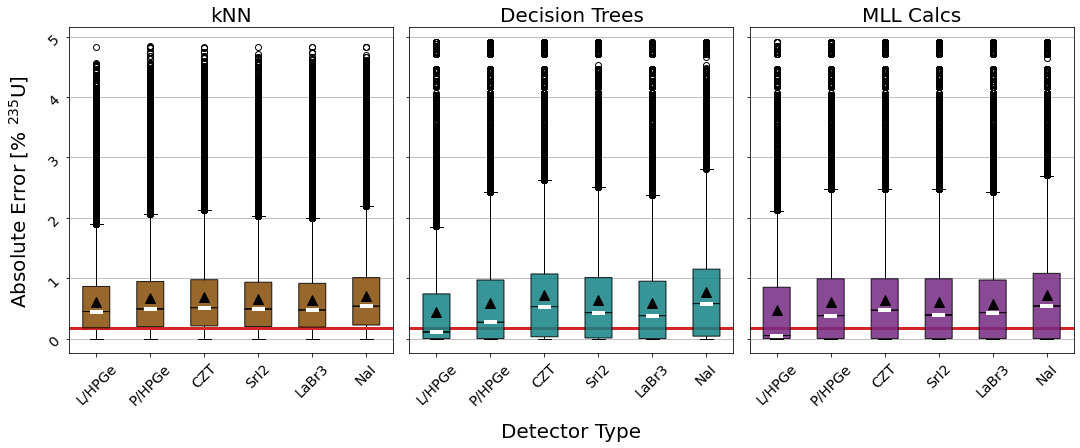
\includegraphics[width=0.92\textwidth]{./chapters/exp2/abserror_boxplots_outliers_long_enri.png}
    \caption{\gls{U235} enrichment prediction error box plots for long energy windows list.}
    \label{fig:enriboxflyC}
  \end{subfigure}
  \caption{Prediction performance of \gls{U235} enrichment for six detectors as 
           shown by box plots.}
  \label{fig:enriboxfly}
\end{figure}

\subsubsection{Time Since Irradiation Regression}

\begin{figure}[!htb]
  \centering
  \begin{subfigure}[b]{\textwidth}
    \centering
    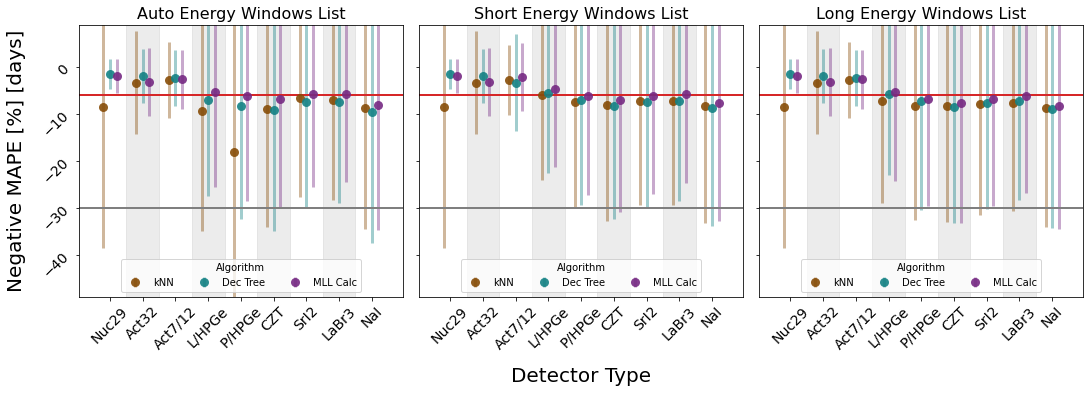
\includegraphics[width=\textwidth]{./chapters/exp2/detector_preds_wrt_enlist_MAPE_cool.png}
    \caption{Time since irradiation prediction performance measured by \gls{MAPE}.}
    \label{fig:coolA}
  \end{subfigure}
  \vskip\baselineskip
  \begin{subfigure}[b]{\textwidth}
    \centering
    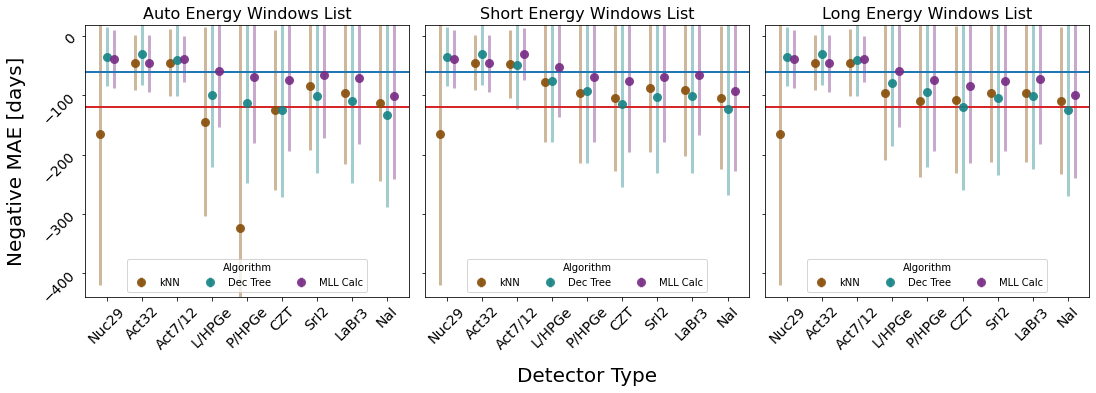
\includegraphics[width=\textwidth]{./chapters/exp2/detector_preds_wrt_enlist_MAE_cool.png}
    \caption{Time since irradiation prediction performance measured by \gls{MAE}.} 
    \label{fig:coolB}
  \end{subfigure}
  \caption{Prediction performance of time since irradiation with respect to 
           decreasing detector energy resolution for three types of processed 
           gamma spectra.}
  \label{fig:cool}
\end{figure}

The goal lines and baselines for the time since irradiation plots in Figure
\ref{fig:cool} were all chosen by the performance of algorithms at a reference
point of 20\% training set error for the 29 nuclide mass training set in in
Figures \ref{fig:randerrD} and \ref{fig:randmaeC}, with one exception where an
arbitrary choice needed to be made.  The \textit{k}-nearest neighbors results
had to be excluded from consideration since the behavior of this algorithm
degraded drastically at 20\% training set error.  For Figure \ref{fig:coolA},
the blue line is at -6\%, which corresponds to the decision trees performance
at the reference point.  The red baseline is at -10\%, which is the previously
mentioned arbitrary choice, since using the \textit{k}-nearest neighbors value
of -30\% would not yeild an interesting discussion.  For Figure
\ref{fig:coolB}, the blue line is at $-60\:days$, and the red baseline is at
$-120\:days$.  The latter corresponds to decision trees at the reference point
in Figure \ref{fig:randmaeC}. The former was informed by the value of \gls{MLL}
at the reference point ($-40\:days$), but made to be a little lower to better
evaluate the detector results, none of which reach a negative error of that
level.  The same lines are present in Figure \ref{fig:coolbox}, but instead are
positive values so the red line is on top.

\begin{figure}[!hp]
  \centering
  \begin{subfigure}[b]{\textwidth}
    \centering
    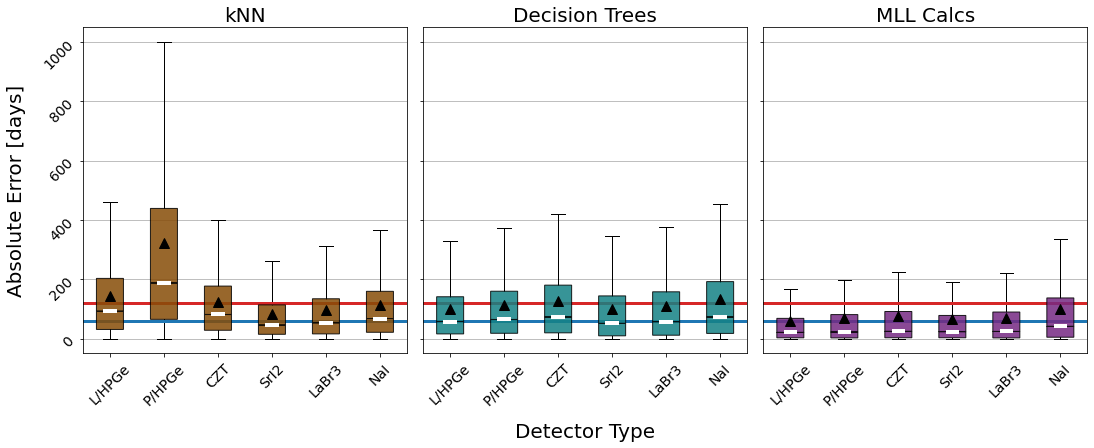
\includegraphics[width=0.92\textwidth]{./chapters/exp2/abserror_boxplots_auto_cool.png}
    \caption{Time since irradiation prediction performance box plots for auto energy windows list.}
    \label{fig:coolboxA}
  \end{subfigure}
  \vskip\baselineskip
  \begin{subfigure}[b]{\textwidth}
    \centering
    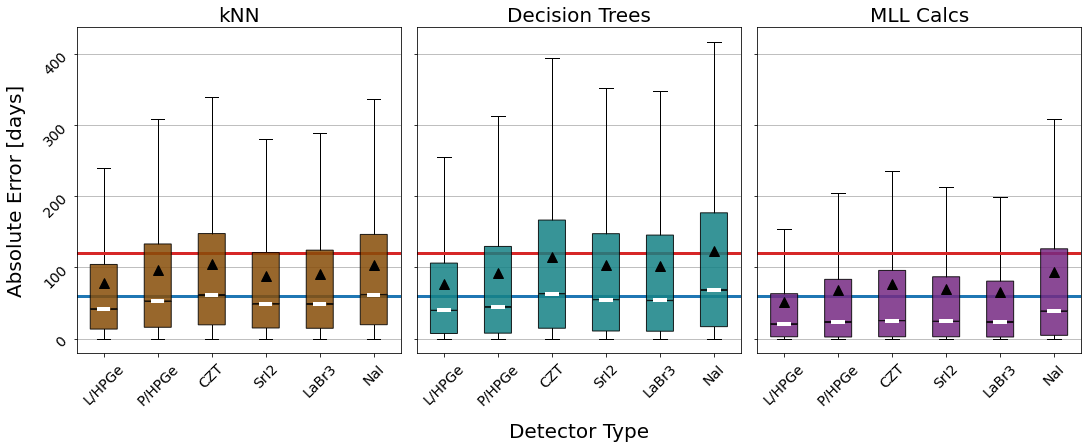
\includegraphics[width=0.92\textwidth]{./chapters/exp2/abserror_boxplots_short_cool.png}
    \caption{Time since irradiation prediction performance box plots for short energy windows list.}
    \label{fig:coolboxB}
  \end{subfigure}
  \vskip\baselineskip
  \begin{subfigure}[b]{\textwidth}
    \centering
    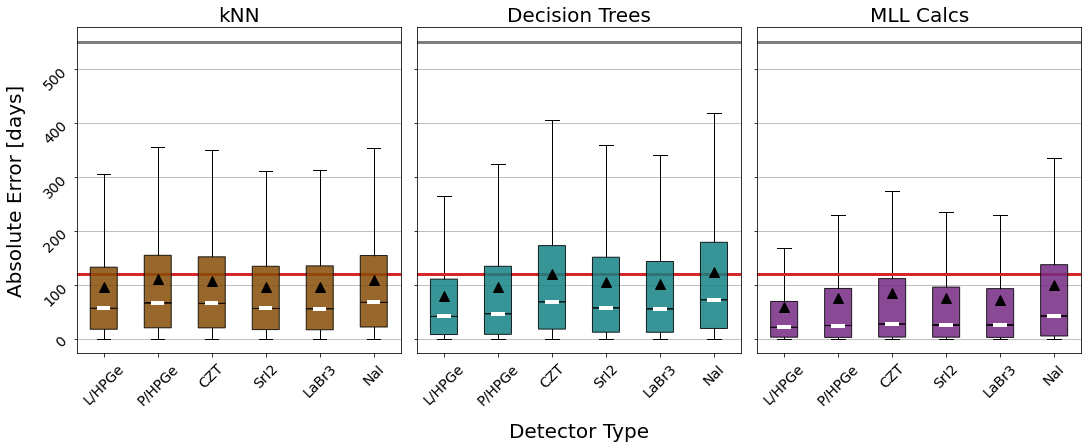
\includegraphics[width=0.92\textwidth]{./chapters/exp2/abserror_boxplots_long_cool.png}
    \caption{Time since irradiation prediction performance box plots for long energy windows list.}
    \label{fig:coolboxC}
  \end{subfigure}
  \caption{Prediction performance of time since irradiation for six detectors as 
           shown by box plots.}
  \label{fig:coolbox}
\end{figure}

\begin{figure}[!hp]
  \centering
  \begin{subfigure}[b]{\textwidth}
    \centering
    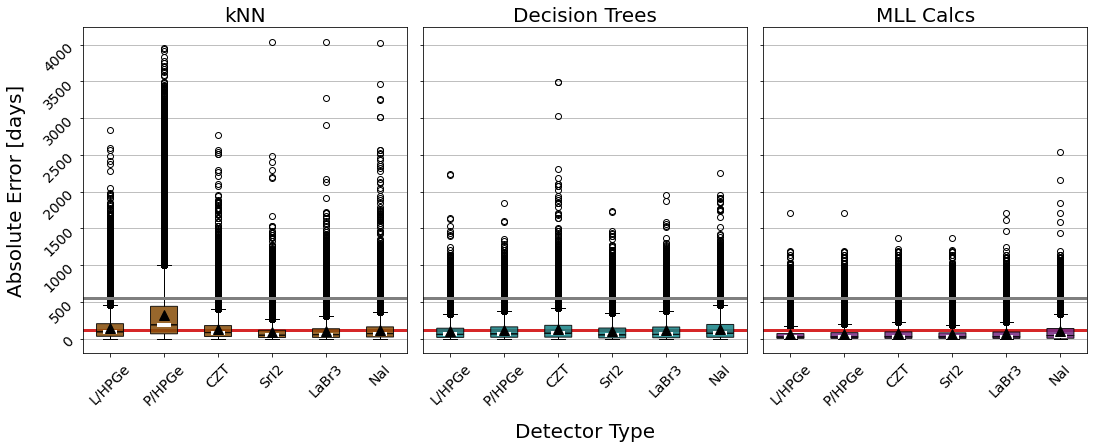
\includegraphics[width=0.92\textwidth]{./chapters/exp2/abserror_boxplots_outliers_auto_cool.png}
    \caption{Time since irradiation prediction performance box plots for auto energy windows list.}
    \label{fig:coolboxflyA}
  \end{subfigure}
  \vskip\baselineskip
  \begin{subfigure}[b]{\textwidth}
    \centering
    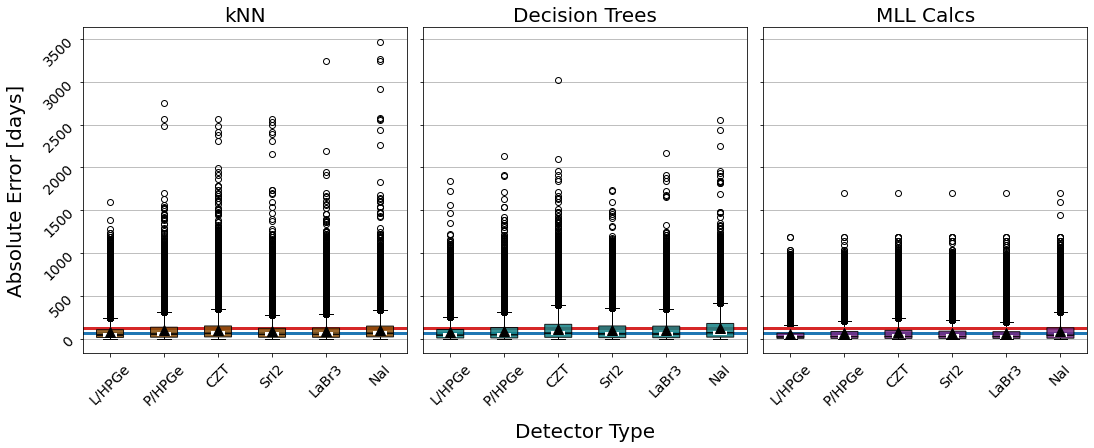
\includegraphics[width=0.92\textwidth]{./chapters/exp2/abserror_boxplots_outliers_short_cool.png}
    \caption{Time since irradiation prediction performance box plots for short energy windows list.}
    \label{fig:coolboxflyB}
  \end{subfigure}
  \vskip\baselineskip
  \begin{subfigure}[b]{\textwidth}
    \centering
    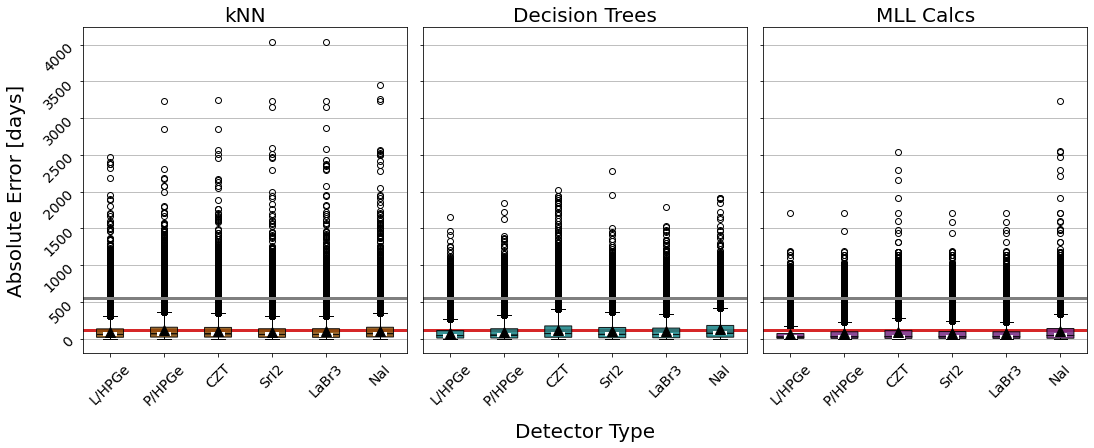
\includegraphics[width=0.92\textwidth]{./chapters/exp2/abserror_boxplots_outliers_long_cool.png}
    \caption{Time since irradiation prediction performance box plots for long energy windows list.}
    \label{fig:coolboxflyC}
  \end{subfigure}
  \caption{Prediction performance of time since irradiation for six detectors as 
           shown by box plots.}
  \label{fig:coolboxfly}
\end{figure}

